\documentclass[utf8]{frontiersSCNS}
\usepackage{gensymb}
\usepackage{url,hyperref,lineno,microtype,subcaption}
\usepackage[onehalfspacing]{setspace}

\linenumbers
\usepackage{wasysym} % provides \DH, \dh, \Thorn, \thorn
% Leave a blank\usepackage{amsmath}
%\DeclareMathOperator{\sign}{sign} line between paragraphs instead of using \\

\usepackage{booktabs}
\usepackage{multirow}
\usepackage{siunitx} %for SI units

\def\keyFont{\fontsize{8}{11}\helveticabold }
\def\firstAuthorLast{Balasubramanian {et~al.}} %use et al only if is more than 1 author
\def\Authors{Suryanarayanan Balasubramanian\,$^{1}$, Martin Hoelzle\,$^{1}$}
\def\Address{$^{1}$University of Fribourg, Department of Geosciences, Fribourg, Switzerland\\} \def\corrAuthor{Suryanarayanan Balasubramanian}

\def\corrEmail{suryanarayanan.balasubramanian@unifr.ch}


\begin{document}
\onecolumn
\firstpage{1}

\title[Artificial Ice Reservoirs]{Optimal discharge rates for artificial ice reservoir (Icestupa) evolution}

\author[\firstAuthorLast ]{\Authors}
\address{}
\correspondance{}

\extraAuth{}

% \maketitle
\begin{abstract}
  Since 2014, mountain communities in Ladakh, India have been constructing dozens of Artificial Ice Reservoirs
  (AIRs) by spraying water through fountain systems every winter. The meltwater from these structures is crucial
  to meet irrigation water demands during spring. However, the water use efficiency (WUE) of this technology is
  poor due to the variability of AIR freezing rates due to the weather and fountain influences at the chosen
  location. This study compares the WUE between an AIR constructed manually with an AIR constructed using
  automated systems at Guttannen, Switzerland. The automation software uses a simplified equation with 6
  coefficients that capture the influence of temperature, humidity, wind and solar radiation variations on the
  freezing rate. Historical meteorological data in conjunction with the coordinates, altitude and time zone of
  the site are required to calculate these 6 coefficients. The automated AIR had a WUE three times more
  than the manual AIR. This is a promising result for dry mountain regions, where automated AIR technology could
  scale current mitigation efforts.

	\tiny
	\keyFont{ \section{Keywords:} icestupa, water storage, climate change adaptation, geoengineering } %All article types: you may provide up to 8 keywords; at least 5 are mandatory.
\end{abstract}

\section{Introduction}

\section{Study Sites and data}

\section{Automation methodology}
\subsection{Model assumptions}

The objective of the automation system is to estimate the optimal discharge rate given weather, fountain and
location information. In order to do so, we simplify the methodology used in our previous paper with some
assumptions. We tend to use assumptions that overestimate the associated freezing rate to optimise more for
maximum ice volume rather than WUE. Below we present each of our assumptions corresponding to the different
model modules in our previous paper.

\subsection{Surface area calculation} \label{sec:shape}

The surface area varies significantly over the lifetime of an AIR. To approximate it, we assume the radius and
the height of the AIR are equal or the slope of the cone is 1. Admittedly, this overestimates the surface area
of the AIR thereby overestimating both its freezing and melting rates. 

\subsection{Energy balance calculation} \label{sec:energy}

\subsubsection{Net Shortwave Radiation \texorpdfstring{$q_{SW}$}{Lg}} \label{sec:SW}
The diurnal variation of the shortwave radiation can be captured via a gaussian equation. However, the seasonal
variations in the amplitude of the solar radiation are poorly captured by such an equation. Since, typical AIRs
have a construction period spanning less than 3 months, we can ignore the seasonal variations of solar
radiation. Therefore, 

\begin{equation}
	Radiation induced melt = \frac{amp}{(\sigma \sqrt{2\pi})} \cdot exp\left(\frac{-(time-\mu)^2}{2\sigma^2}\right)
	\label{eqn:auto}
\end{equation}

\subsubsection{Net Longwave Radiation \texorpdfstring{$q_{LW}$}{Lg}} \label{sec:LW}

\subsection{Automation equation}

The automation equation is composed of two parts namely, (a) linear and (b) gaussian equation. (a)
approximates the influence of temperature, wind speed and humidity on the expected freezing rate. (b)
approximates the contribution of solar radiation on the expected freezing rates. 

\begin{equation}
	\frac{\Delta M_{F}}{\Delta t} = a \cdot T_a + b \cdot RH + c \cdot v_a + d
  +\frac{amp}{(\sigma \sqrt{2\pi})} \cdot exp\left(\frac{-(time-\mu)^2}{2\sigma^2}\right)
	\label{eqn:auto}
\end{equation}

\section{Results}

\begin{figure}
	\begin{center}
		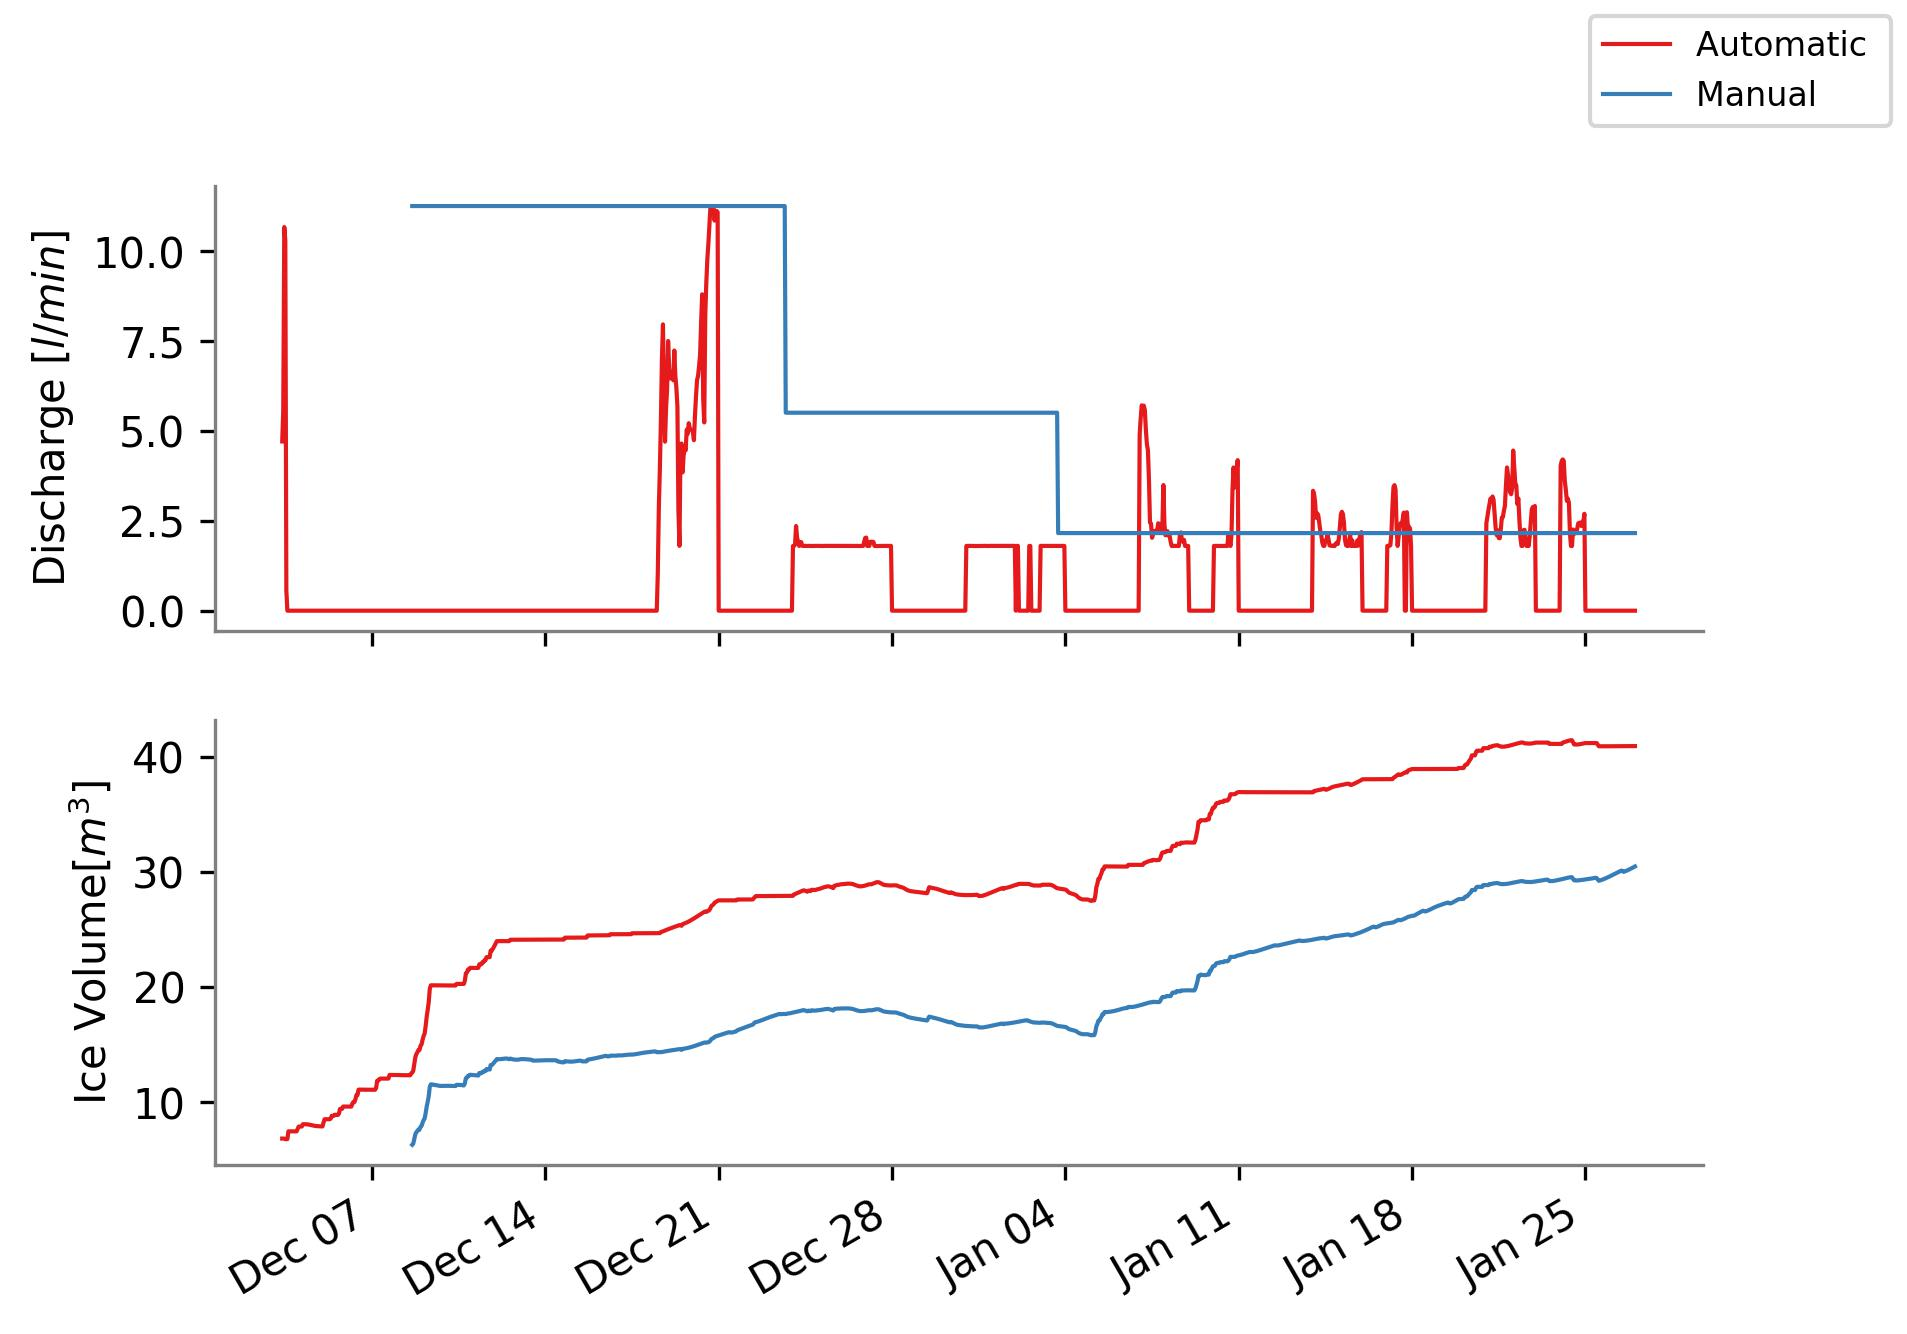
\includegraphics[width=\linewidth]{Figures/autovsmanual.jpg}
	\end{center}
	\caption{Icestupa in Ladakh, India on March 2017 was 24 $m$ tall and contained around 3700 $m^3$
		of water. Picture Credits: Lobzang Dadul}
	\label{fig:old_icestupa}
\end{figure}

\subsection{Validation}

\section{Discussion}

\section{Conclusions}

\section{Appendix}

\end{document}
